%% LyX 2.3.5.2 created this file.  For more info, see http://www.lyx.org/.
%% Do not edit unless you really know what you are doing.
\documentclass[11pt,english]{article}
\usepackage[utf8x]{luainputenc}
\usepackage{geometry}
\geometry{verbose,headheight=110pt}
\usepackage{fancyhdr}
\pagestyle{fancy}
\usepackage{amsmath}
\usepackage{amsthm}
\usepackage{amssymb}

\makeatletter
%%%%%%%%%%%%%%%%%%%%%%%%%%%%%% User specified LaTeX commands.


% add LaTeX packages to use here
\usepackage{amsfonts}
\usepackage{amsthm}
\usepackage{fancyhdr}
\usepackage{lastpage}
\usepackage{enumitem}
\usepackage{framed}
\usepackage[most]{tcolorbox}
\usepackage{graphicx}
\usepackage{tikz}
\usepackage{forest}
\usepackage[english]{babel}
\usepackage{tikz-qtree}
% set dimensions for page layout


\setlist[itemize]{leftmargin=*} % prevents indenting of itemize

% abbreviations for some common math symbols
\newcommand{\Rset}{\hbox{$\mathbb R$}}
\newcommand{\Nset}{\hbox{$\mathbb N$}}
\newcommand{\Pset}{\hbox{$\mathbb{N}^{+}$}}
\newcommand{\Zset}{\hbox{$\mathbb N$}}
\newcommand{\Qset}{\hbox{$\mathbb Q$}}

% theorem style
\newtheoremstyle{thmstyle}% name of the style to be used
  {0pt}% measure of space to leave above the theorem. E.g.: 3pt
  {0pt}% measure of space to leave below the theorem. E.g.: 3pt
  {}% name of font to use in the body of the theorem
  {}% measure of space to indent
  {\bfseries}% name of head font
  {.}% punctuation between head and body
  { }% space after theorem head; " " = normal inter-word space
  {}% Manually specify head

% theorem environment instance
\theoremstyle{thmstyle}
\newtheorem{theorem}{Theorem}

% shaded and framed solution environment 

\newenvironment{shadedSolutionBox}{\setlength{\OuterFrameSep}{0in}%
  \definecolor{shadecolor}{gray}{.8}% shading of shaded solution box
  \bigskip%
  \@nameuse{shaded*}\par\noindent\ignorespaces \textit{Solution}.}{\hspace{\stretch{1}}\rule{1.5ex}{1.5ex}% adds filled box 
  \@nameuse{endshaded*}%
  \bigskip}


% shaded and framed theorem environment 

\newenvironment{thm}{\setlength{\OuterFrameSep}{0in}%
  \definecolor{shadecolor}{gray}{1}% shading of shaded Theorem box
  \@nameuse{snugshade*}\par\noindent\ignorespaces%
   \@nameuse{theorem}}{\hspace{\stretch{1}}\scalebox{1.5}{\hbox{$\triangleleft$}}% adds triangle shape
  \@nameuse{endtheorem}%
  \@nameuse{endsnugshade*}%
  }


% header and footer elements of every page except the first.

\fancyfoot[L]{\textsc{CSc {\small\selectfont 30400}} }
\fancyhead[R]{{\small\selectfont\textsc{\studentLastName}}}
\fancyfoot[C]{{\small\selectfont\assignmentName}}
\fancyfoot[R]{{\small\selectfont\thepage\ of \pageref{LastPage}}}
\renewcommand{\headrulewidth}{0.8pt}
\renewcommand{\footrulewidth}{0.4pt}

% hline with variable thickness

\def\thickhline{%
  \noalign{\ifnum0=`}\fi\hrule \@height \thickarrayrulewidth \futurelet
   \reserved@a\@xthickhline}
\def\@xthickhline{\ifx\reserved@a\thickhline
               \vskip\doublerulesep
               \vskip-\thickarrayrulewidth
             \fi
      \ifnum0=`{\fi}}


% length instance for \thickhline
\newlength{\thickarrayrulewidth} 
\setlength{\thickarrayrulewidth}{.8pt}

% header and footer for first page
\fancypagestyle{firstpage}
{
\fancyhf{}
\renewcommand{\footrulewidth}{0.4pt}
\renewcommand{\headrulewidth}{0pt}
\fancyhead[C]{%
\begin{tabular*}{\textwidth}{@{\extracolsep{\fill}}@{}l @{} c @{} r @{} }
{\small\selectfont\courseName}&{\normalsize\selectfont\assignmentName}&{\small\selectfont\studentFirstName\ \studentLastName}\\
\thickhline
&&{\scriptsize\selectfont\collaboratorNames}
\end{tabular*}%
}
\fancyfoot[R]{{\small\selectfont\thepage\ of \pageref{LastPage}}}
\fancyfoot[L]{{\footnotesize\selectfont\pdfcreationdate}}
}

\newcommand{\courseName}{Theoretical Computer Science} % course name

% your first name, your last name, and the assignment name
\newcommand{\studentLastName}{Luka} % your last name
\newcommand{\studentFirstName}{Nikabadze} % your first name (and middle name, if applicable)
\newcommand{\assignmentName}{Homework5} % the assignment name
\newcommand{\collaboratorNames}{[B]. Nikabadze} % if you worked with anyone to complete any part of the assignment, include the initial of the first name (and middle name, if applicable) and full last name of each of your collaborators, separated by commas (e.g., if you worked with Arthur Paul Pedersen and Sandra Lee, include "A.P. Pedersen, S. Lee")

\makeatother

\usepackage{babel}
\begin{document}
% marks the beginning of the document

\thispagestyle{firstpage} % institutes page style for first page

\setlength{\abovedisplayskip}{20pt} % space above math in align* environment
\setlength{\belowdisplayskip}{20pt} % space below math in align* environment

% marks the beginning of the document body

\setlength{\itemsep}{1em} % \itemsep is the spacing between items in environment

\begin{itemize}
\item[1.]

Here the FA contains many epsilon transition.

But finally the last 2 symbol which has to be there in the string so that the automata accepts it is ba.

When the second last symbol is b , it is on the 3rd last state. Then since the transition is epsilon , it goes to the second last state with out any symbol and then finally accepts a and go to final state.

Thus the last two symbol has to be ba.

In the string , aabbaba the last 2 symbol is ba. Thus it is accepted by the automata while in the string aabbabb the last two symbol is ba. It will never go to final state. Thus it is not accepted by the automata.

\end{itemize}


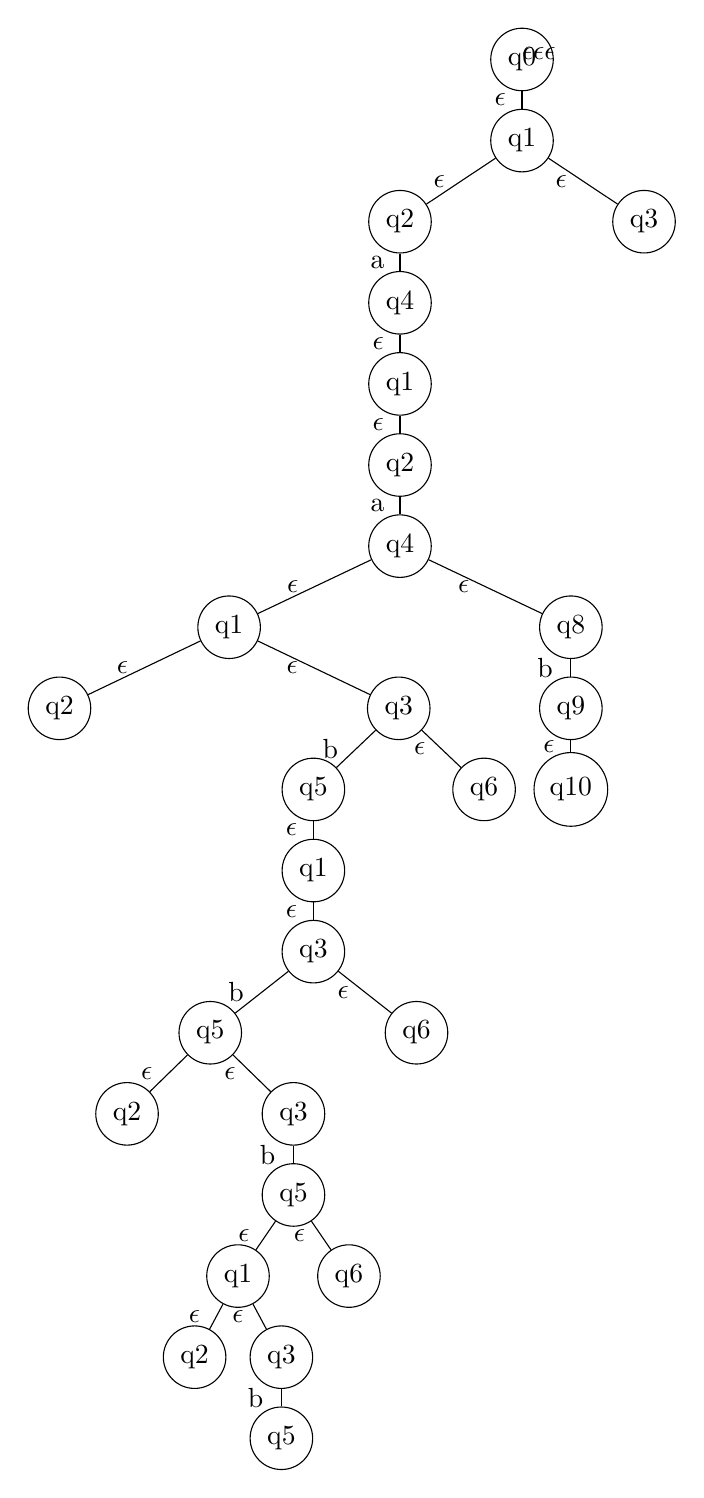
\begin{tikzpicture}[every tree node/.style=draw,circle,
   level distance=1.03cm,sibling distance=.05cm,
   edge from parent path=(\tikzparentnode) -- (\tikzchildnode)]
\Tree
[.q0
    \edge node[auto=right] {$\epsilon$};
    [.q1
       \edge node[midway,left] {$\epsilon$};
       [.q2
        \edge node[midway,left] {a};
            [.q4 
                \edge node[midway,left] {$\epsilon$};
                    [.q1
                        \edge node[midway,left] {$\epsilon$};
                            [.q2 
                                \edge node[midway,left] {a};
                                [.q4
                                    \edge node[midway,left] {$\epsilon$};
                                    [.q1
                                        \edge node[midway,left] {$\epsilon$};
                                        [.q2 ]
                                        \edge node[midway,left] {$\epsilon$};
                                        [.q3
                                           \edge node[midway,left] {b};
                                           [.q5
                                            \edge node[midway,left] {$\epsilon$};
                                            [.q1 
                                                \edge node[midway,left]  {$\epsilon$};
                                                [.q3 
                                                \edge node[midway,left] {b};
                                                [.q5 
                                                \edge node[midway,left]  {$\epsilon$};
                                                    [.q2 ]
                                                     \edge node[midway,left] {$\epsilon$};
                                                     [.q3
                                                        \edge node[midway,left] {b};
                                                        [.q5
                                                         \edge node[midway,left] {$\epsilon$};
                                                         [.q1 
                                                         \edge node[midway,left] {$\epsilon$};
                                                         [.q2 ]
                                                         \edge node[midway,left] {$\epsilon$};
                                                         [.q3
                                                         \edge node[midway,left] {b};
                                                         [.q5 ]
                                                         ]
                                                         ]
                                                         \edge node[midway,left] {$\epsilon$};
                                                         [.q6 ]
                                                        ]
                                                     ]
                                                ]
                                                \edge node[midway,left] {$\epsilon$};
                                                [.q6 ]
                                                ]
                                                ]
                                                ]
                                                \edge node[midway,left] {$\epsilon$};
                                                [.q6 ]
                                                ]
                                                ]
                                                \edge node[midway,left]  {$\epsilon$};
                                                [.q8
                                                    \edge node[midway,left] {b};
                                                    [.q9 
                                                    \edge node[midway,left] {$\epsilon$};
                                                        [.q10 ]
                                                    ]
                                                ]
                                                ]
                                            ]
                                           ]
                                        ]
                                    ]
                                    \edge node[midway,left] {$\epsilon$};
                                    [.q3 ]
                                ]
                            ]
                            \edge node[midway,left] {$\epsilon$};
                            [.q3 ]
                    ]
                    \edge node[midway,left] {$\epsilon$};
                    [.q6
                                 
                                ]
                           ] 
                       ]
                    ]
            ]
       ]
       \edge node[midway,left] {$\epsilon$};
       [.q3 ]
    ]
]
\end{tikzpicture}




\begin{tikzpicture}[every tree node/.style=draw,circle,
   level distance=1.03cm,sibling distance=.05cm,
   edge from parent path=(\tikzparentnode) -- (\tikzchildnode)]
\Tree
[.q0
    \edge node[auto=right] {$\epsilon$};
    [.q1
       \edge node[midway,left] {$\epsilon$};
       [.q2
        \edge node[midway,left] {a};
            [.q4 
                \edge node[midway,left] {$\epsilon$};
                    [.q1
                        \edge node[midway,left] {$\epsilon$};
                            [.q2 
                                \edge node[midway,left] {a};
                                [.q4
                                    \edge node[midway,left] {$\epsilon$};
                                    [.q1
                                        \edge node[midway,left] {$\epsilon$};
                                        [.q2 ]
                                        \edge node[midway,left] {$\epsilon$};
                                        [.q3
                                           \edge node[midway,left] {b};
                                           [.q5
                                           \edge node[midway,left]   {$\epsilon$};
                                            [.q2 ]
                                            [.q4 
                                            \edge node[midway,left] {b};
                                            [.q5
                                            \edge node[midway,left]   
                                            [.q7 ]
                                            ]
                                            ]
                                            ]
                                            ]
                                            \edge node[midway,left]  {$\epsilon$};
                                            [.q3 
                                            \edge node[midway,left] {a};
                                            [.q6
                                            \edge node[midway,left] {a};
                                                [.q7 
                                                \edge node[midway,left] {$\epsilon$};
                                                [.q8
                                                    \edge node[midway,left] {b};
                                                    [.q9 
                                                    \edge node[midway,left] {$\epsilon$};
                                                        [.q10
                                                        \edge node[midway,left] {$\epsilon$};
                                                        [.q11 ]
                                                        ]
                                                    ]
                                                ]
                                                ]
                                            ]
                                            ]
                                           ]
                                           ]
                                           ]
                                        ]
                                    ]
                                    \edge node[midway,left] {$\epsilon$};
                                    [.q3 ]
                                ]
                            ]
                            \edge node[midway,left] {$\epsilon$};
                            [.q3 ]
                    ]
                    \edge node[midway,left] {$\epsilon$};
                    [.q6
                       \edge node[midway,left] {a};
                       [.q7 
                          \edge node[midway,left] {$\epsilon$};
                           [.q8 
                            \edge node[midway,left] {b};
                                [.q9
                                  \edge node[midway,left] {$\epsilon$};
                                    [.q10 ]
                                ]
                           ] 
                       ]
                    ]
            ]
       ]
       \edge node[midway,left] {$\epsilon$};
       [.q3 ]
    ]
]
\end{tikzpicture}


2. Use Nerode's equivalance relation to show that language $a^{*}b^{*}$
is regular and the language $\{a^{n}b^{n}|n\in N\}$ is not. What
about language $\{a^{n}b^{*}|n\in N\}$

In order to show that the Language L = a*b* is regular we show that L has only 3 equivalence classes:

$[\epsilon]:$ This consists of all the strings in the Language.

$[b]:$ Any string of the form bn is in this class.

$[\phi]$: All strings not in L.

Since L has only 3 equivalence classes, L is regular.

The language $L = {anbn | n>=0}$ as it has infinite equivalence classes:

1) $[\epsilon]:$ consisting of strings in L

2) $[a]$: consisting of strings of the form $an-1bn$

3) $[a^2]$: consisting of strings of the form $an-2bn$

4) and so on

Hence the language is not regular.

The language $L = \{a^nb^* | n \in N\}$ is regular as it is same as the language $a+b*$.

\end{document}
